\newpage
\section{Durchführung und Versuchsaufbau}

\subsection{Versuchsaufbau}

\noindent Der Versuchsaufbau besteht aus dem in Abbildung \ref{img:aufbau} dargestellten Gerät. 
Die wichtigsten Bauteile sind dabei die links zu sehende Kupfer-Röntgenröhre, der LiF-Kristall für die Bragg-Reflexion und dem Geiger-Müller-Zählrohr.\\
Das abgebildete Röntgengerät ermöglicht die Aufnahme der Spektren übder einen Computer.
\begin{figure}[ht]
    \centering
    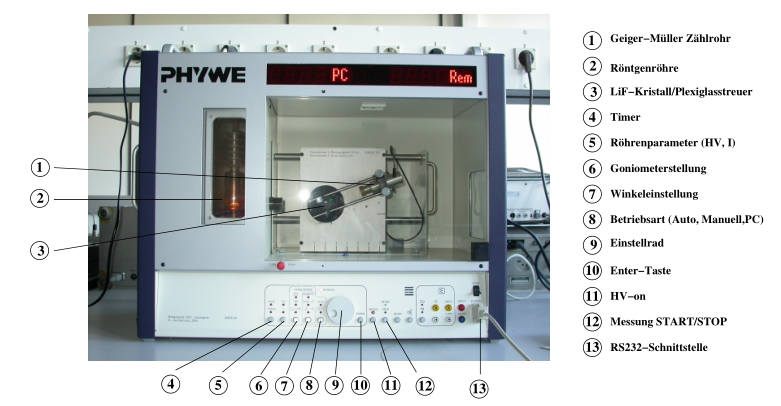
\includegraphics[width=0.7\textwidth]{latex/images/aufbau.PNG}
    \caption{Der Versuchsaufbau der zur Untersuchung der Röntgenstrahung genutzt wird. Dabei sind die einzelnen Komponenten in der Legende aufgeschlüsselt. \protect \cite{V401}.}
    \label{img:aufbau}
\end{figure}

\noindent Dafür muss auf dem Computer das Programm \enquote*{measure} ausgeführt und darin das Röntgengerät ausgewählt werden.\\
Die zu wählenden Einstellungen sind die Messart \enquote*{Spektren}, die Beschleunigungsspannung $U_B=\SI{35}{\kilo\volt}$ und der Emissionstrom $I=\SI{1}{\milli\ampere}$.\\
Die Weiteren für Einstellung benötigten Knöpfe sind in der Legende von Abbildung \ref{img:aufbau} aufgeführt.


\subsection{Bragg'sche Bedingung}

In der ersten Messreihe soll die Bragg'sche Bedingung untersucht werden. 
Dafür wird der Winkel des Kristalls auf $\theta=\SI{14}{\degree}$ gestellt und anschließend die Winkeleinstellung des Geiger-Müller-Zählrohrs von $\alpha_{GM}=\SI{26}{\degree}$ bis $\alpha_{GM}=\SI{30}{\degree}$ variiert.
Dabei soll für die Integrationszeit $\increment t=\SI{5}{\second}$ und für den Winkelzuwachs $\increment \alpha=\SI{0.1}{\degree}$ gewählt werden.\\
Des Weiteren sollte der LiF-Kristall und eine $\SI{1}{\milli\metre}$ Blende noch in das Röntgengerät eingesetzt werden.
Der Koppelmodus sollte auf 2:1 gestellt werden.\\
Anschließend soll der mit dem gemessenen Maximum korrespondierende Winkel mit dem Glanzwinkel verglichen werden und bei zu großen Abweichungen die assistierende Person benachrichtigt werden.

\subsection{Emissionspektrum der Kupfer-Röntgenröhre}

\noindent
Hier wird nur die Schrittweite auf $\increment \theta=\SI{0.2}{\degree}$ geändert und der Winkelbereich des Kristalls von $\theta=\SI{4}{\degree}$ bis $\theta=\SI{26}{\degree}$ variiert.\\
Im aufgenommenen Spektrum sollen dann, zusätzlich zu den charakteristischen Linien und derm Bremsberg, die minimale Wellenlänge identifiziert werden.\\\\
Anschließend soll noch das Detailspektrum der $K_{\alpha}$ und $K_{\beta}$ aufgenommen werden, wobei $\increment \theta=\SI{0.1}{\degree}$ und $\increment t=\SI{5}{\second}$ seien sollen.\\
Aus dieser Messung soll dann die Halbwertsbreite der Linien berechnet werden und damit dann im weiteren das Auflösevermögen der Apparatur.\\
Zuletzt sollen die Abschirmkonstanten $\sigma_1$, $\sigma_2$ und $\sigma_3$, unter Vernachlässigung des Drehimpulsbeitrags, aus den Emissionsenergien berechnet werden. \\
Die Konstanten können dann mit folgenden Gleichungen und Literaturwerten für die Energien abgeschätzt werden. Dabei ist $n=1$, $m=2$ und $l=3$.
\begin{align*}
    E_{K,abs}&=\symup{R_\infty}(z-\sigma_1)^2\\
    E_{K,\alpha}&=\symup{R_\infty}\frac{1}{n^2}(z-\sigma_1)^2-\symup{R_\infty}\frac{1}{m^2}(z-\sigma_2)^2\\
    E_{K,\beta}&=\symup{R_\infty}\frac{1}{n^2}(z-\sigma_1)^2-\symup{R_\infty}\frac{1}{l^2}(z-\sigma_3)^2
\end{align*}

\subsection{Absorptionsspektrum}

In diesem Versuchsabschnitt wird ein Zinkabsorber vor das Zählrohr gesetzt und $\increment \theta=\SI{0.1}{\degree}$ und $\increment t=\SI{20}{\second}$.\\
Aus den damit generierten Messwerten soll die Absorptionsenergie der K-Kante berechnet werden. Hieraus kann nun die Abschirmzahl von Zink $\sigma_K$ bestimmt werden.\\
Dies kann nun mit den vier weiteren Absorbern Brom, Gallium, Rubidium und Strontium wiederholt werden.\\
Zuletzt soll mit den Absorptionsenergien das Moseleysche Gesetz überprüft werden.\\
Dieses besagt, dass $E_K$ proportional zum Quadrat der Ordnungszahl $Z^2$ ist. Dies soll über ein $\sqrt{E_K}$-$Z$ Diagramm bestimmt werden, wo die Steigung die Rydberg-Konstante seien soll. 